\documentclass{beamer}
\usepackage{xeCJK}
\usepackage[xjtu,zh]{collegeBeamer}
\usepackage{booktabs}

\setCJKmainfont[
    Path = C:/Users/10451/AppData/Local/Microsoft/Windows/Fonts/,
    BoldFont = SourceHanSerifSC-Bold.otf,
]{SourceHanSerifSC-Regular.otf}
% when using Chinese, uncomment the following line
% \usepackage{xeCJK}

% meta-data
\title{金属电子逸出功虚拟仿真实验报告}
\subtitle{物理实验大作业报告}
\author{吉致贤\\梅现\\吴政豪}
\date{报告日期:2024.12.29}

% document body
\begin{document}
    
    \maketitle

    \begin{frame}
    本次汇报主要介绍测量金属逸出功和磁控法测量电子荷质比,及两个实验的实验原理,以及展示我们的实验仿真软件。

    我们利用matlab GUI搭建仿真实验平台,平台共包含三个部分:实验测量界面、金属逸出功数据处理界面和电子荷质比数据处理界面。
    
    实验测量界面中,用户可来回切换两个实验,用户可调控灯丝电流、励磁电流和阳极电压,得到阳极电流和灯丝温度,同时用户还可观察到电子的运动过程。用户可将测量数据输入到数据处理界面,得到金属逸出功和电子荷质比的实验值,并附有数据图像展示。
    \end{frame}

    \section{实验原理}
    \subsection{金属逸出功原理}
    \begin{frame}{理查森-杜西曼公式}{\thesubsection \, \subsecname}
        \begin{columns}[T]
            \begin{column}{0.5\textwidth}
                如图所示,用钨丝作阴极的理想二极管,通以电流加热,并在阳极和阴极间加上正向电压时,在外电路中就有电流通过。电流的大小主要与灯丝温度及金属逸出功的大小有关。
                
                根据费米-狄拉克分布可以导出热电子发射遵守的\textbf{理查森-杜西曼公式}:
                \begin{equation}
                    I = AST^2\exp(-\frac{e\varphi}{kT})
                \end{equation}
            \end{column}
            \begin{column}{0.3\textwidth}
                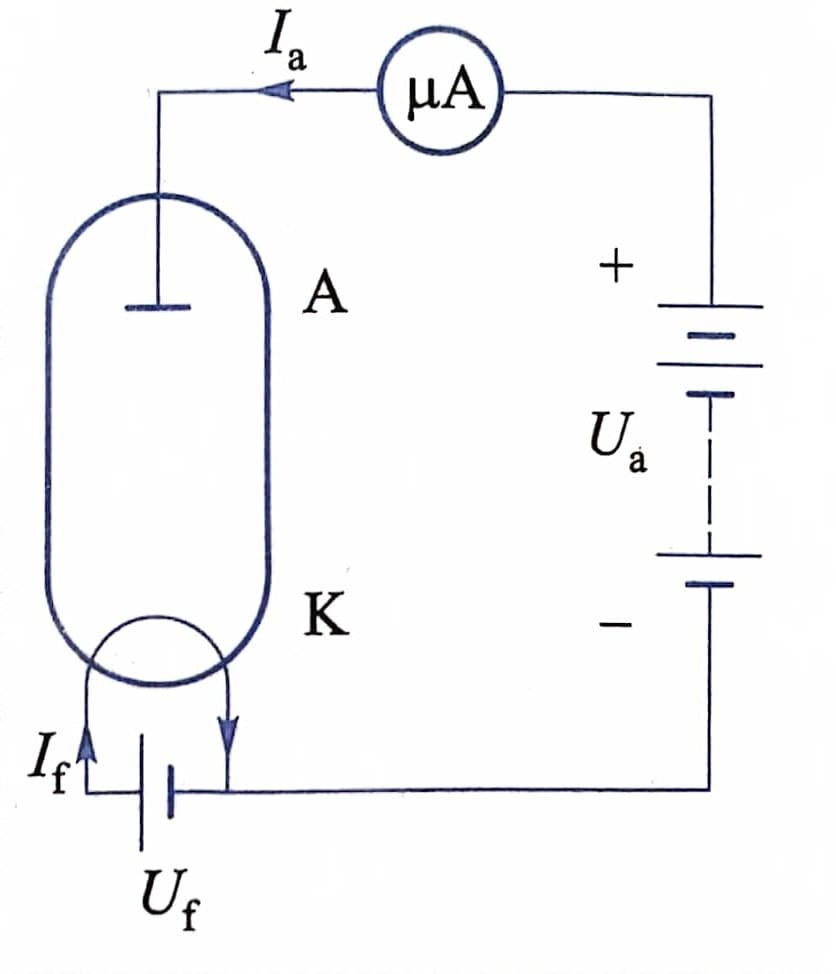
\includegraphics[scale=0.2]{gallery/pic1.jpg}
                
            \end{column}
        \end{columns}
    \end{frame}

    \begin{frame}{理查森直线法}{\thesubsection \, \subsecname}
        从上式可知,只要测出I、A、S、T的值,就可以计算出阴极材料的电子逸出功,但是直接测定 A、S 这两个量比较困难。故我们采用理查森直线法,它可以避开 A、S 的测量,即不必求出 A、S 的具体数值,直接由发射电流 I 和灯丝温度 T 确定逸出功的值。

        由式(1)得到式(2):
        \begin{equation}
            \frac{I}{T^2} = AS\exp(-\frac{e\varphi}{kT})
        \end{equation}

        两边取常用对数得到:
        \begin{equation}
            \lg\frac{I}{T^2} = \lg AS - \frac{e\varphi}{2.303k}\cdot \frac{1}{T}
        \end{equation}
    \end{frame}

    \begin{frame}{灯丝温度}{\thesubsection \, \subsecname}
        灯丝温度对发射电流I的影响很大,因此准确测量灯丝温度对于减小测量误差非常重要。若不测量灯丝温度,可以根据灯丝真实温度与灯丝电流的关系,由灯丝电流确定灯丝温度,钨丝的真实温度与加热电流的对应关系如下表所示。
        \begin{table}
            \footnotesize
            \caption{钨丝的真实温度与加热电流的对应关系}
            \centering
            \begin{tabular}{cccccccccc}
            \toprule
            \textbf{灯丝电流}/A & 0.600	& 0.625	& 0.650	& 0.675	& 0.700	& 0.725	& 0.750	& 0.775	& 0.800\\
            \midrule
            \textbf{灯丝温度}/(103K) & 1.88	& 1.92	& 1.96	& 2.00	& 2.04	& 2.08	& 2.12	& 2.16	& 2.20\\
            \bottomrule
            \end{tabular}
        \end{table}
    \end{frame}

    \begin{frame}{金属逸出功原理}{\thesubsection \, \subsecname}
        要使阴极发射的热电子连续不断地飞向阳极,形成阳极电流$I_a$,就必须在阳极与阴极之间外加一个加速电场$E_a$。

        阴极发射电流$I_a$与阴极表面加速电场$E_a$的关系是式(4):
        \begin{equation}
            I_a = I \exp(\frac{\sqrt{e^3E_a}}{kT})
        \end{equation}
        式中,$I_a$和$I$分别表示加速电场为$E_a$和零时的发射电流。
    \end{frame}

    \begin{frame}{金属逸出功原理}{\thesubsection \, \subsecname}
        为了方便,一般将阴极和阳极制成共轴圆柱体,在忽略接触电势差等影响的条件下,阴极表面附近加速电场的场强为式(5)
        \begin{equation}
            E_a = \frac{U_a}{r_1\ln(\frac{r_2}{r_1})}
        \end{equation}
        式中,$r_1$、$r_2$分别为阴极及阳极圆柱面的半径,$U_a$为加速电压。

        将式(4)代入式(5)取对数得
        \begin{equation}
            \lg I_a = \lg I + \frac{\sqrt{e^3}}{2.303kT}\cdot \sqrt{\frac{U_a}{r_1\ln(\frac{r_2}{r_1})}}
        \end{equation}
    \end{frame}

    \begin{frame}{金属逸出功原理}{\thesubsection \, \subsecname}
        综上所述,要测定某金属材料的逸出功,可将该材料制成理想二极管的阴极,测定阴极温度$T$、阳极电压$U_a$和发射电流$I_a$,用作图法得到零场电流$I$后,即可求出逸出功或逸出电势。
    \end{frame}

    \subsection{磁控法测电子荷质比原理}

    \begin{frame}{磁控法测电子荷质比原理}{\thesubsection \, \subsecname}
        在一定的阳极电压下,阳极电流$I_a$与励磁电流$I_r$的关系,在开始阶段几乎不发生改变,随着励磁电流$I_r$的逐渐增加,$I_a$的变化曲率达到最大.之后,随着$I_r$的加大,$I_a$逐步减小,平降到0。在$I_a$-$I_r$曲线上取阳极电流最大值$I_a$约1/4高度的点作为阳极电流变化的临界点$Q$,临界点$Q$只是个统计的概念,实际上不同速率运动的电子的临界点是不同的。
    \end{frame}

    \begin{frame}{磁控法测电子荷质比原理}{\thesubsection \, \subsecname}
        在单电子近似的情况下,从阴极发射出的、质量为$m$的电子动能应有阳极加速电场能$eU_a$和灯丝加热后电子“热运动”所具能量$W$两部分构成,所以有式(7)
        \begin{equation}
            \frac{1}{2}mv^2 = eU_a + W
        \end{equation}
        电子在磁场$B$的作用下做半径为$R$的圆周运动,应满足式(8)
        \begin{equation}
            eBv = \frac{mv}{R}
        \end{equation}
        通电励磁线圈中心处的磁感应强度有式(9)
        \begin{equation}
            B = \frac{\mu_0NI_s}{2(r_2-r_1)}\ln \frac{r_2+\sqrt{r_2^2+L^2}}{r_1+\sqrt{r_1^2+L^2}} = K'I_s
        \end{equation}
        其中,$r_1$为线圈的内半径;$r_2$为线圈的外半径;$L$为线圈半长度;$K'$为比例分数。
    \end{frame}

    \begin{frame}{磁控法测电子荷质比原理}{\thesubsection \, \subsecname}
        由式(7)、(8)、(9)可得式(10)
        \begin{equation}
            \frac{U_a+W/e}{I_s^2} = \frac{e}{m} \cdot \frac{R^2}{2}\cdot K'^2
        \end{equation}
        若设阳极内半径为$a$,而阴极(灯丝)半径忽略不计,则当多数电子都处于临界状态,与临界点$Q$对应的励磁线圈的电流$I_a$称为临界电流$I_c$,而此时$R = a/2$,阳极电压$U_a$与$I_c$的关系可写为式(11)
        \begin{equation}
            \frac{U_a+W/e}{I_c^2} = \frac{e}{m} \cdot \frac{a}{8}\cdot K'^2 = K
        \end{equation}
    \end{frame}

    \begin{frame}{总结}{\thesubsection \, \subsecname}
        用同一个理想二极管,在不同的$U_a$下,就有不同的阳极电流与励磁电流变化曲线,因而就有不同的$I_c$值与之对应。再将测得的$U_a$-$I_c^2$数据组用图解法或最小二乘法球的斜率$K$,从而求得电子荷质比。
    \end{frame}

    \section{仿真软件展示}
    \begin{frame}{测量页面}{\thesection \, \secname}
        \begin{columns}[T]
            \begin{column}{0.4\textwidth}
                下面是我们仿真实验平台的展示:

                平台共包含三个部分,实验测量页面,金属逸出功的数据处理页面和电子荷质比数据处理页面,通过点击最上方按钮切换三种页面。
            \end{column}
            \begin{column}{0.3\textwidth}
                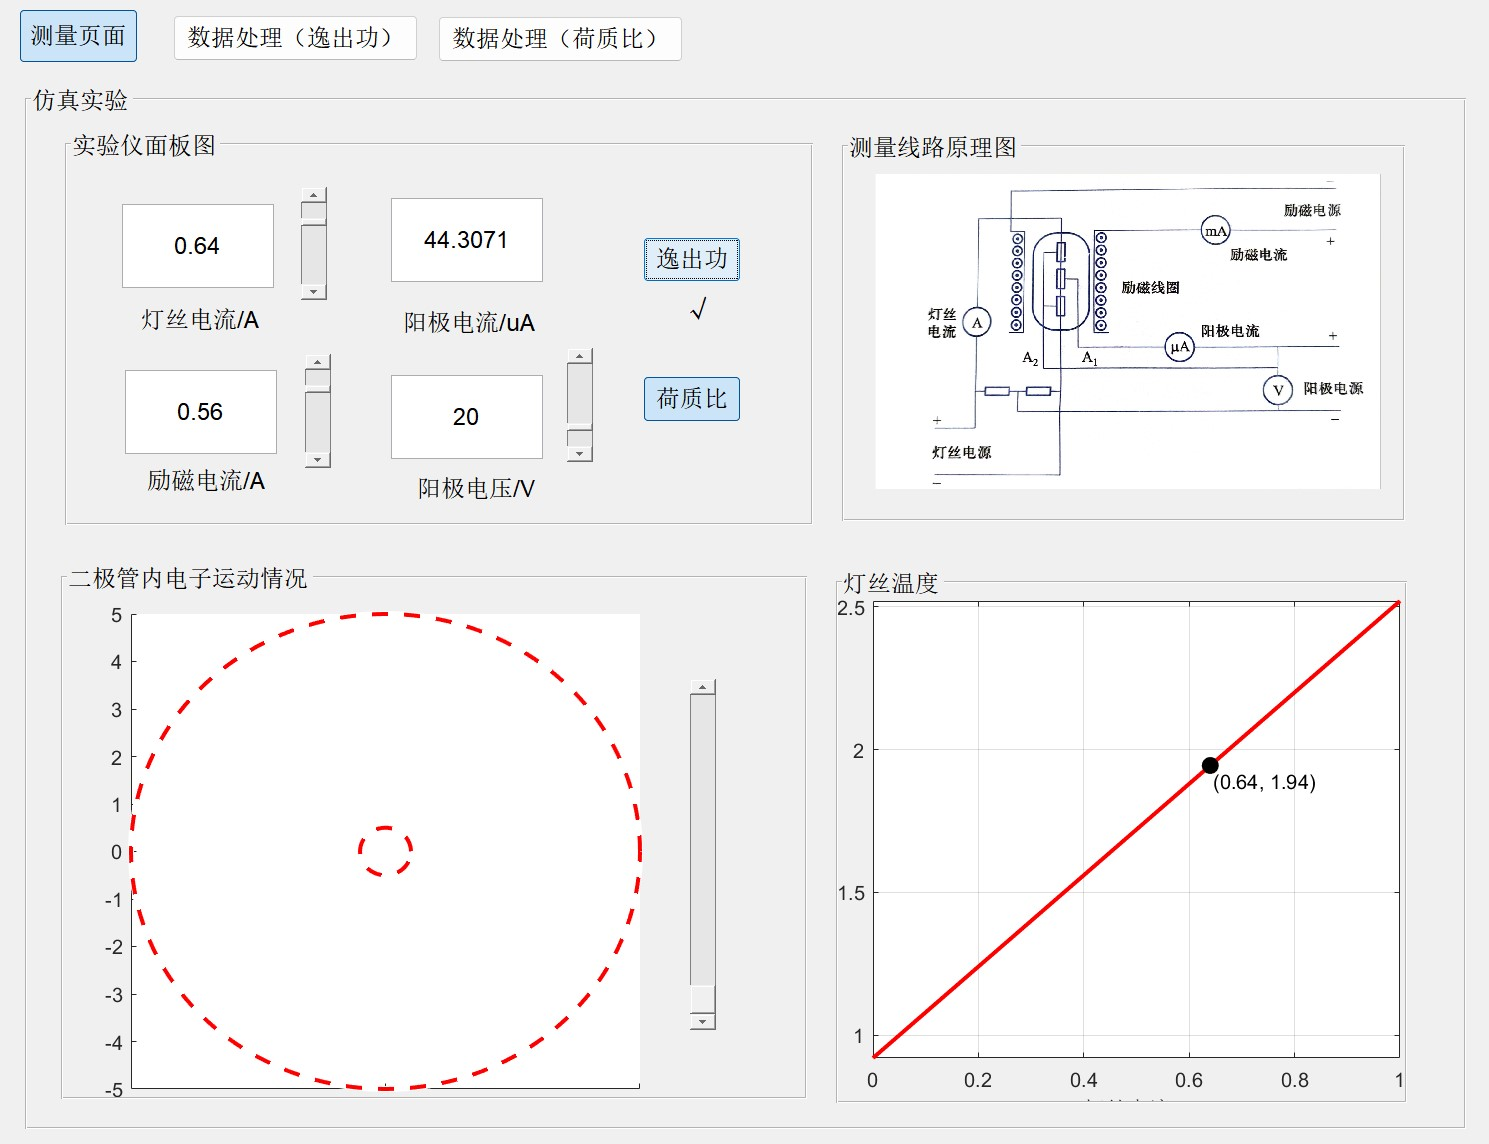
\includegraphics[scale=0.22]{gallery/pic3.jpg}
            \end{column}
        \end{columns}
        
    \end{frame}

    \begin{frame}{测量页面}{\thesection \, \secname}
        \begin{columns}
            \begin{column}{0.3\textwidth}
                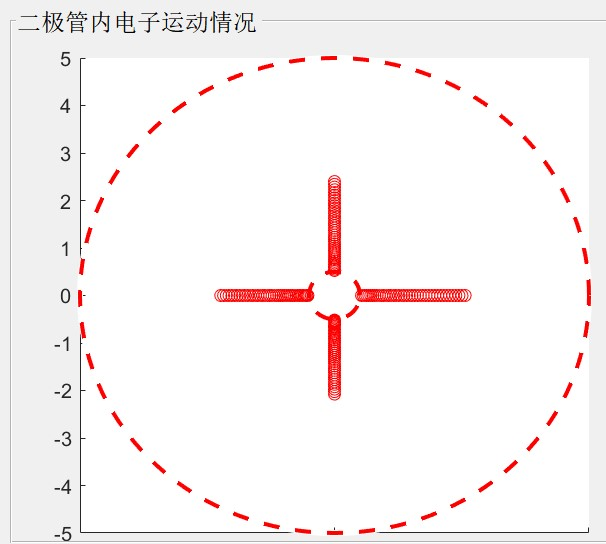
\includegraphics[scale=0.35]{gallery/move1.jpg}
                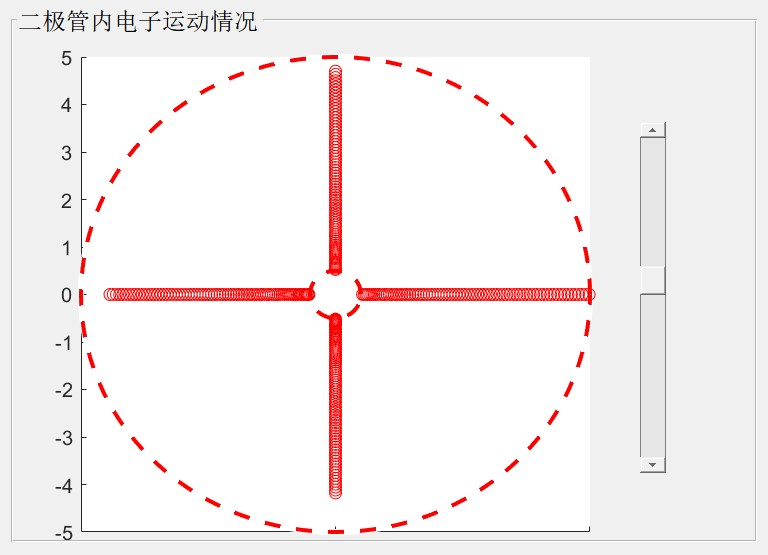
\includegraphics[scale=0.35]{gallery/move2.jpg}
            \end{column}
            \begin{column}{0.3\textwidth}
                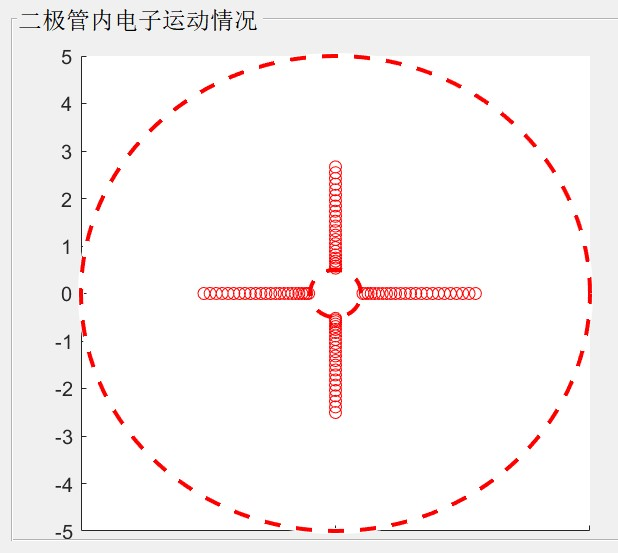
\includegraphics[scale=0.35]{gallery/move3.jpg}
                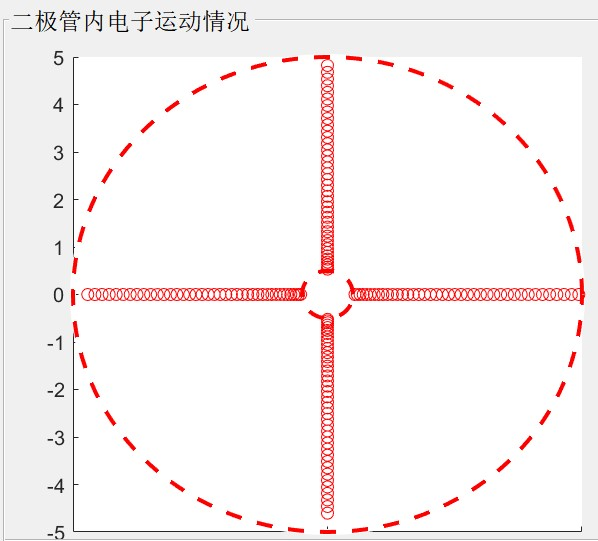
\includegraphics[scale=0.35]{gallery/move4.jpg}
            \end{column}
        \end{columns}
    \end{frame}

    \begin{frame}{测量页面}{\thesection \, \secname}
        \begin{columns}
            \begin{column}{0.3\textwidth}
                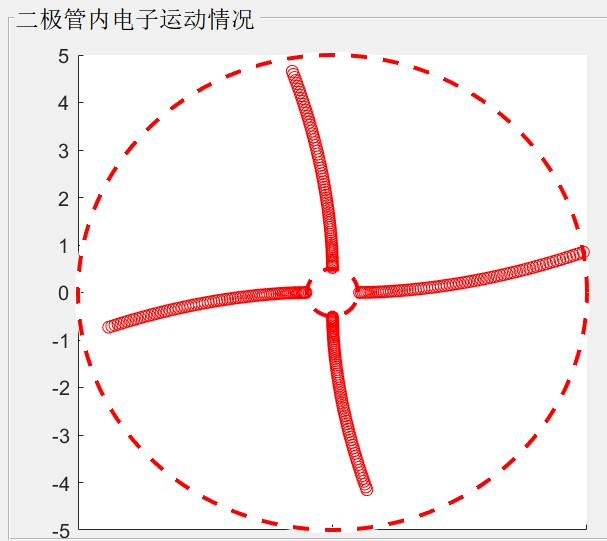
\includegraphics[scale=0.35]{gallery/move5.jpg}
                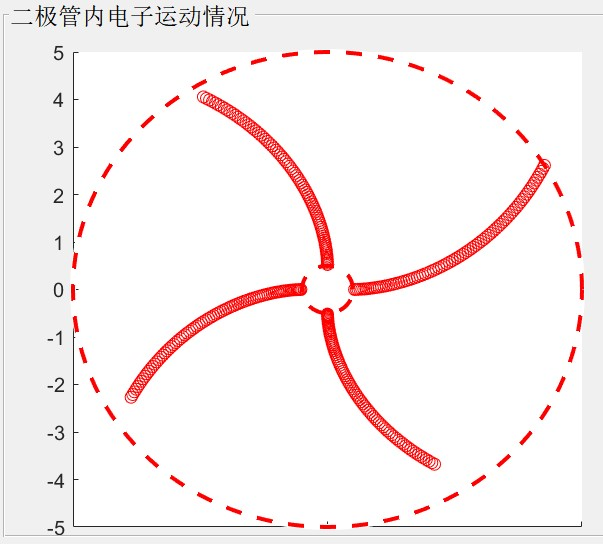
\includegraphics[scale=0.35]{gallery/move6.jpg}
            \end{column}
            \begin{column}{0.3\textwidth}
                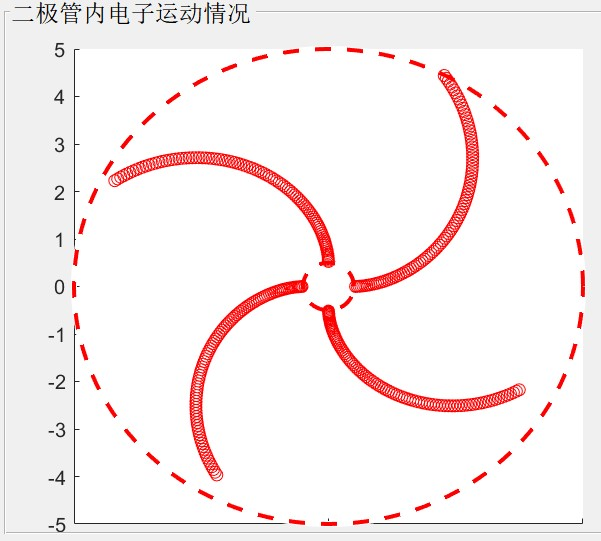
\includegraphics[scale=0.35]{gallery/move7.jpg}
                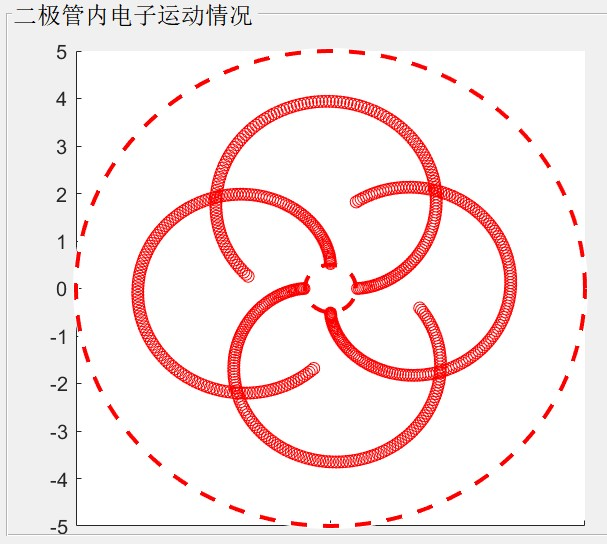
\includegraphics[scale=0.35]{gallery/move8.jpg}
            \end{column}
        \end{columns}
    \end{frame}

    \begin{frame}{数据处理页面(逸出功)}{\thesection \, \secname}
        第二个界面为金属逸出功的数据处理页面:
        \begin{figure}
            \centering
            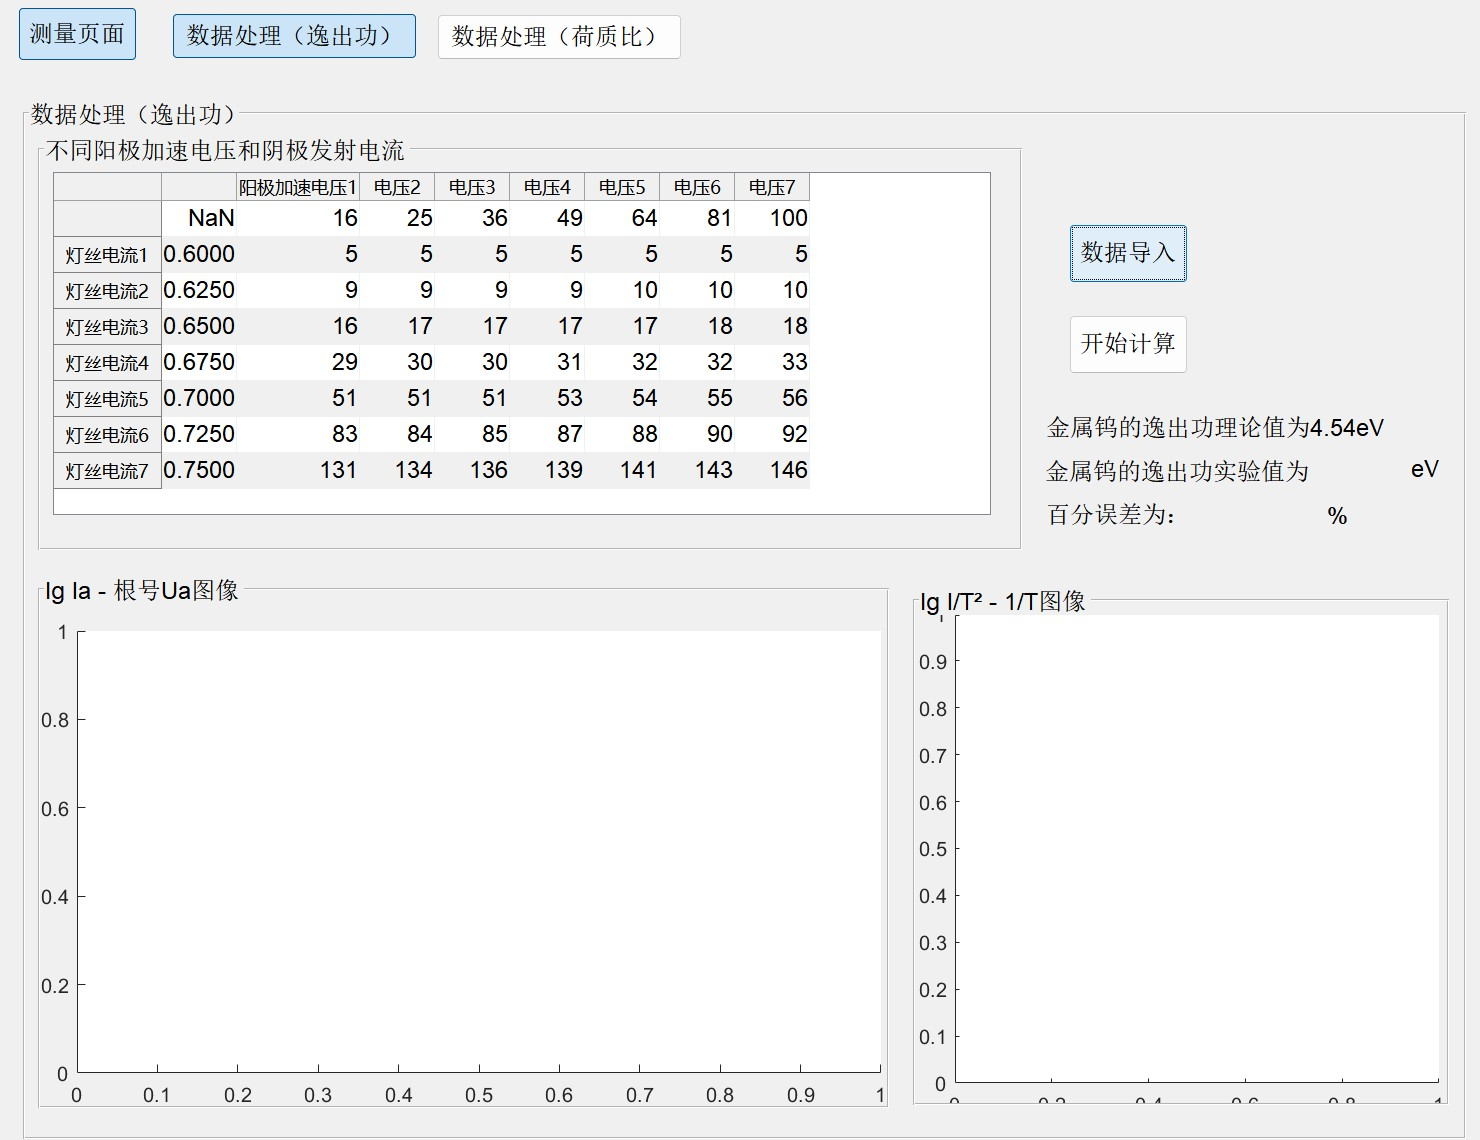
\includegraphics[scale=0.28]{gallery/pic4.jpg}
        \end{figure}
    \end{frame}
    \begin{frame}{数据处理页面(逸出功)}{\thesection \, \secname}
    用户可以点击“数据导入”按钮,导入实验数据,也可以在此基础上手动修改数据。

    点击“开始计算”按钮后,平台将会计算金属逸出功的实验值,给出与理论值的相对误差,并且采用最小二乘法,绘制出$\lg I_a$-$\sqrt{U}$图像和$\lg \frac{I}{T^2}$-$\frac{1}{T}$图像,方便用户检查数据。

        \begin{columns}
            \begin{column}{0.4\textwidth}
                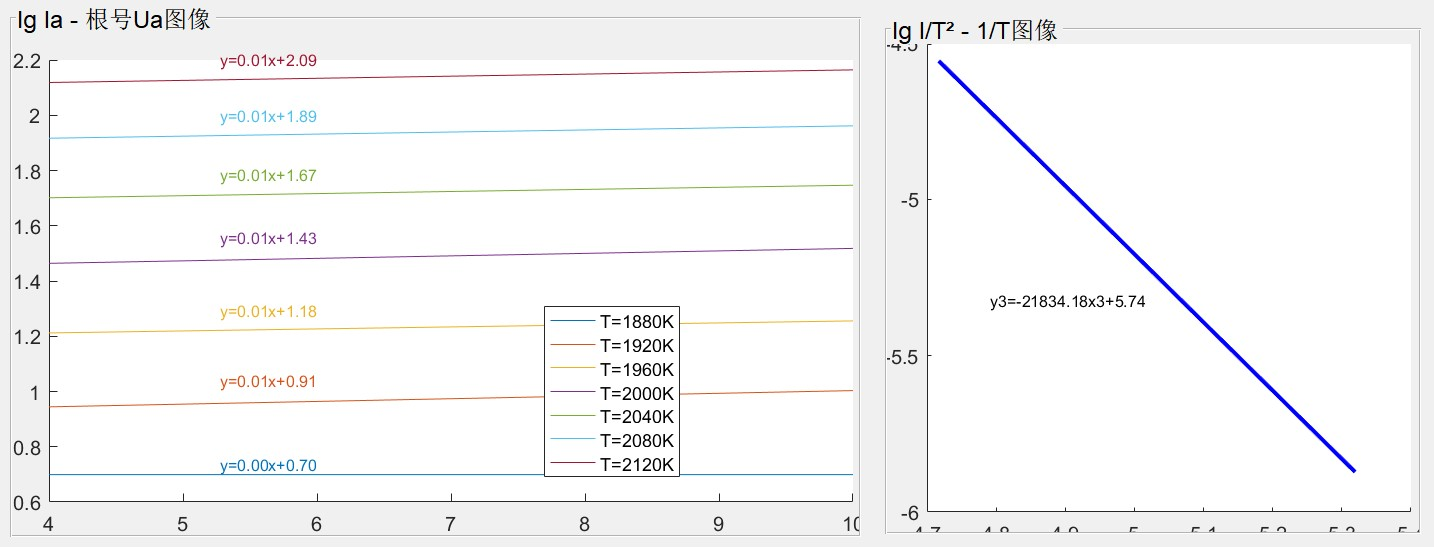
\includegraphics[scale=0.27]{gallery/pic5.jpg}
            \end{column}
            \begin{column}{0.4\textwidth}
                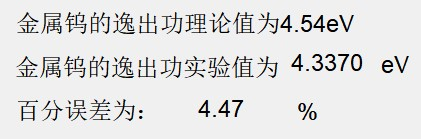
\includegraphics[scale=0.8]{gallery/pic6.jpg}
            \end{column}
        \end{columns}
    \end{frame}

    \begin{frame}{数据处理页面(荷质比)}{\thesection \, \secname}
        第三个页面为电子荷质比的数据处理页面:
        \begin{figure}
            \centering
            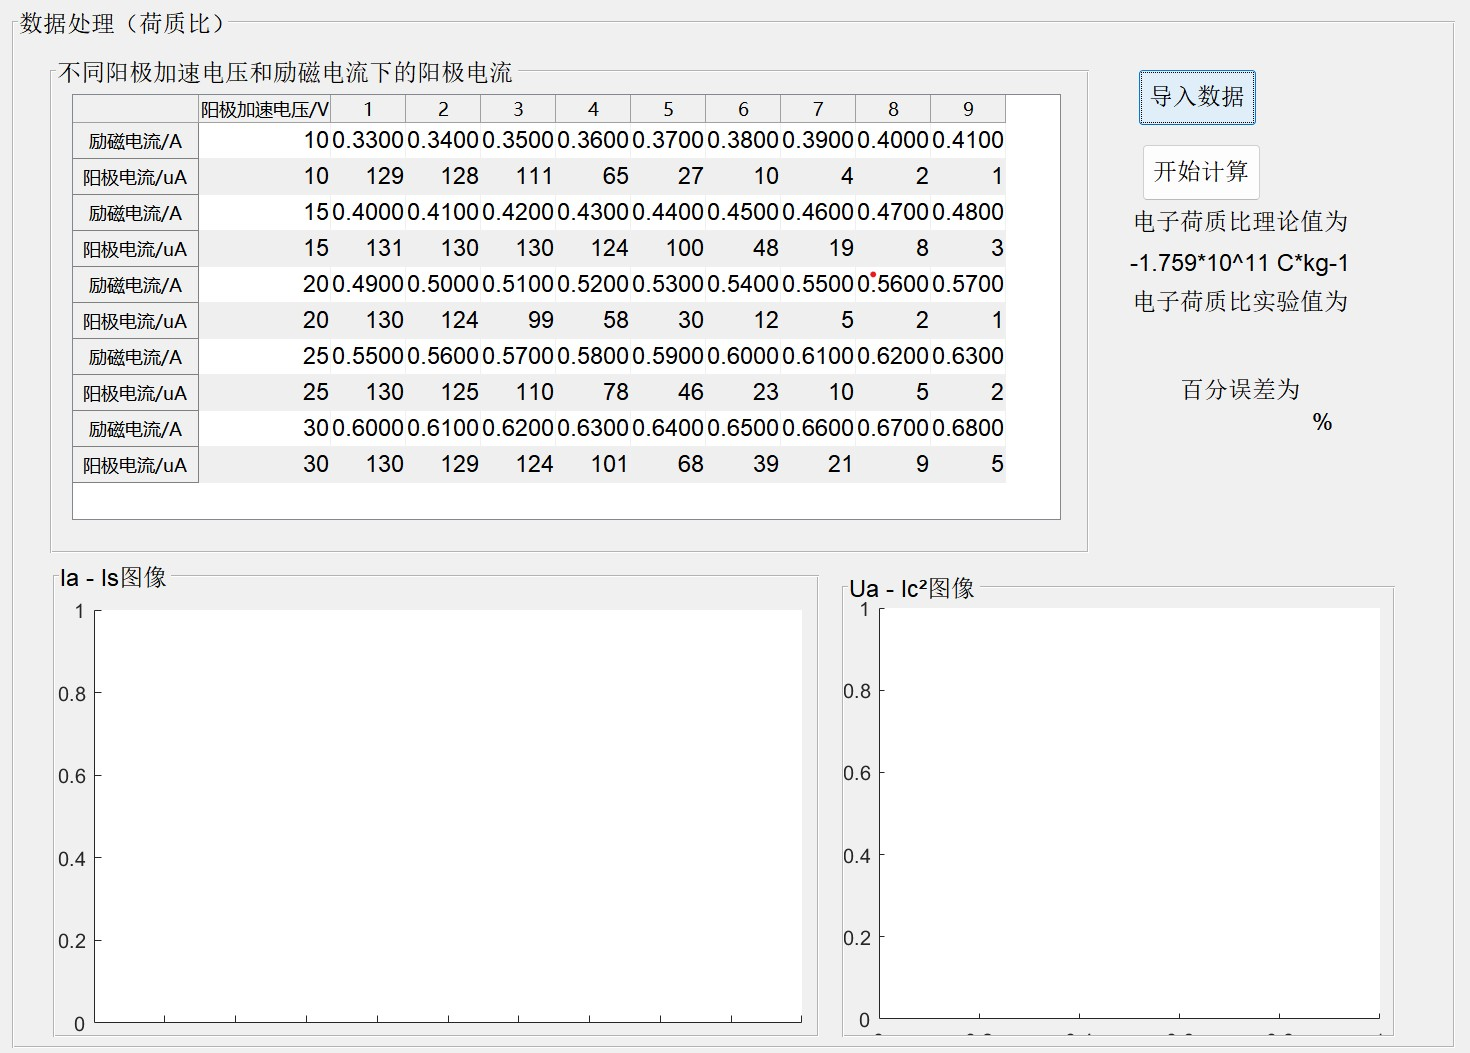
\includegraphics[scale=0.28]{gallery/pic7.jpg}
        \end{figure}
    \end{frame}
    \begin{frame}{数据处理页面(荷质比)}{\thesection \, \secname}
    用户可以点击“数据导入”按钮,导入实验数据,也可以在此基础上手动修改数据。

    点击“开始计算”按钮后,平台将会计算电子荷质比的实验值,给出与理论值的相对误差,并且绘制出$I_a$-$I_s$图像,取最大值的1/4处为临界电流$I_c$,并绘制阳极电压与临界电流平方$U_a$-$I_c^2$图,方便用户检查数据。

        \begin{columns}
            \begin{column}{0.4\textwidth}
                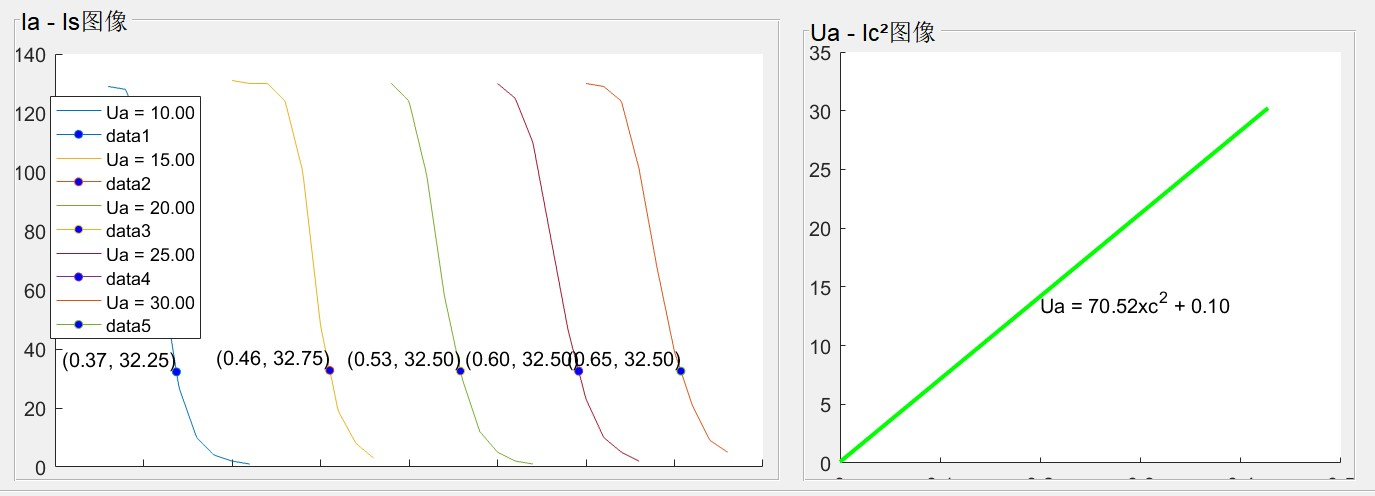
\includegraphics[scale=0.27]{gallery/pic8.jpg}
            \end{column}
            \begin{column}{0.4\textwidth}
                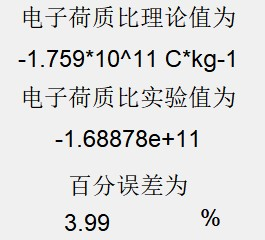
\includegraphics[scale=0.8]{gallery/pic9.jpg}
            \end{column}
        \end{columns}
    \end{frame}
\end{document}